\documentclass{beamer}
\usetheme{CambridgeUS}
\setbeamercolor{block title}{bg=red!80!black, fg=white}
\setbeamercolor{block body}{bg=red!10, fg=black}
%%%%%%%%%%%%%%%%%%%%%%%%%%%%%%%%%%%%%%%%%%%%%%%%%%%%%%%
\usepackage[utf8]{vietnam}
\usepackage{graphicx}
\usepackage{hyperref}
\usepackage{lipsum}
\usepackage{tikz}
%%%%%%%%%%%%%%%%%%%%%%%%%%%%%%%%%%%%%%%%%%%%%%%%%%%%%%%
% \AtBeginSection[]
% {
% \begin{frame}<beamer>
% \frametitle{Nội dung}

% \tableofcontents[
% currentsection,
% subsectionstyle=hide/hide,
% subsubsectionstyle=hide/hide
%]

% \end{frame}
%}
%%%%%%%%%%%%%%%%%%%%%%%%%%%%%%%%%%%%%%%%%%%%%%%%%%%%%%%
% \AtBeginSubsection[]
% {
% \begin{frame}<beamer>
% \frametitle{Nội dung}

% \tableofcontents[
% currentsection,
% currentsubsection,
% subsectionstyle=show/shaded/hide,
% %
% % subsubsectionstyle=hide/hide
% subsubsectionstyle=show/show/shaded/hide
%]

% \end{frame}
%}
%%%%%%%%%%%%%%%%%%%%%%%%%%%%%%%%%%%%%%%%%%%%%%%%%%%%%%%
% \title[{\makebox[.15\paperwidth]{MI4100 - Mật mã và độ phức tạp thuật toán}}]{Chủ đề: Mô phỏng tấn công hệ mật mã khóa công khai RSA bằng thuật toán LLL giảm lưới}
% \author[Nhóm 8]{Nhóm 8}
% \date[\today]{\today}
%%%%%%%%%%%%%%%%%%%%%%%%%%%%%%%%%%%%%%%%%%%%%%%%%%%%%%%
\begin{document}
%%%%%%%%%%%%%%%%%%%%%%%%%%%%%%%%%%%%%%%%%%%%%%%%%%%%%%%
% % Trang tiêu đề
% % Cần có hình ảnh pictures/HUST2.jpeg
% % Không chỉnh sửa gì
% \begin{frame}
% \begin{tikzpicture}[remember picture, overlay]
% \node[anchor=center, inner sep=0pt] at (current page.center) {
\includegraphics[width=\paperwidth, height=\paperheight]{pictures/HUST2.jpeg}};
% \fill[white, opacity=0.8] (current page.south west) rectangle (current page.north east);
% \end{tikzpicture}
% \titlepage
% \end{frame}
%%%%%%%%%%%%%%%%%%%%%%%%%%%%%%%%%%%%%%%%%%%%%%%%%%%%%%%
% \begin{frame}{Danh sách thành viên}
% \begin{block}{Nhóm 8}
% \centering
% \begin{tabular} {|l|c|}
% \hline
% Họ và tên & MSSV \\
% \hline
% Vũ Văn Nghĩa & 20206205 \\
% Vũ Văn Nghĩa & 20206205 \\
% Vũ Văn Nghĩa & 20206205 \\
% Vũ Văn Nghĩa & 20206205 \\
% Vũ Văn Nghĩa & 20206205 \\
% \hline
% \end{tabular}
% \end{block}
% \end{frame}
%%%%%%%%%%%%%%%%%%%%%%%%%%%%%%%%%%%%%%%%%%%%%%%%%%%%%%%
% \begin{frame}{Phân công thành viên}
% \begin{block}{Phân công}
% \begin{itemize}
% \item Vũ Văn Nghĩa: Lập kế hoạch, phân chia công việc
% \item Vũ Văn Nghĩa: Lập kế hoạch, phân chia công việc
% \item Vũ Văn Nghĩa: Lập kế hoạch, phân chia công việc
% \item Vũ Văn Nghĩa: Lập kế hoạch, phân chia công việc
% \item Vũ Văn Nghĩa: Lập kế hoạch, phân chia công việc
% \end{itemize}
% \end{block}
% \end{frame}
%%%%%%%%%%%%%%%%%%%%%%%%%%%%%%%%%%%%%%%%%%%%%%%%%%%%%%%
%! %%%%%%%%%%%%%%%%%%%%%%%%%%%%%%%%%%%%%%%%%%%%%%%%%%%%%%
%! %%%%%%%%%%%%%%%%%%%%%%%%%%%%%%%%%%%%%%%%%%%%%%%%%%%%%%
%! %%%%%%%%%%%%%%%%%%%%%%%%%%%%%%%%%%%%%%%%%%%%%%%%%%%%%%
%! %%%%%%%%%%%%%%%%%%%%%%%%%%%%%%%%%%%%%%%%%%%%%%%%%%%%%%
%! %%%%%%%%%%%%%%%%%%%%%%%%%%%%%%%%%%%%%%%%%%%%%%%%%%%%%%
\section{Tổng quan về hệ mật mã khóa công khai}
\subsection{Lịch sử}
\begin{frame}{Lịch sử}

\begin{itemize}
\item Hệ mật mã khóa công khai là một bước tiến lớn và là cuộc cách mạng trong lĩnh vực mật mã.
\item Hệ mật mã khóa công khai được Diffie và Hellman đưa ra năm 1976.
\end{itemize}

\begin{columns}

\begin{column}{0.4\textwidth}
\begin{figure}[H]
\centering
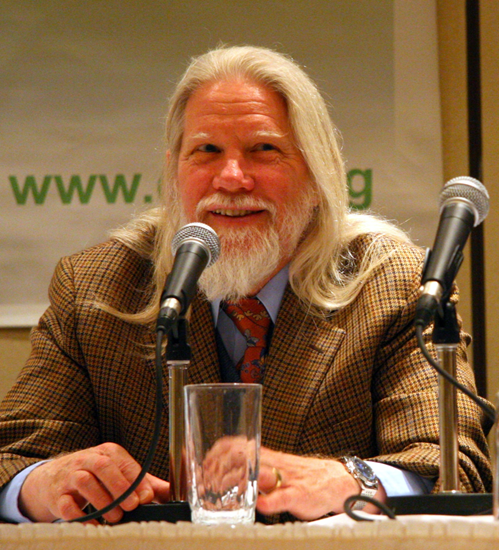
\includegraphics[scale = 0.4]{pictures/Bailey_Whitfield_Diffie.png}
% 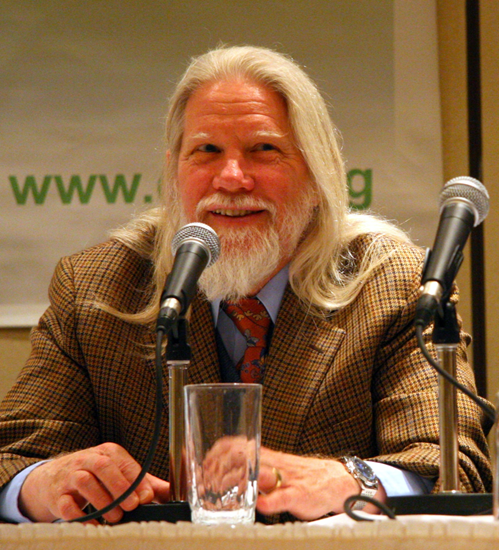
\includegraphics[scale = 0.15]{pictures/Bailey_Whitfield_Diffie.png}
% \caption{Bailey Whitfield 'Whit' Diffie
% (sinh 05/06/1944 – 80 tuổi)
%}
\end{figure}
Bailey Whitfield 'Whit' Diffie\\ (sinh 05/06/1944 – 80 tuổi)
\end{column}

\begin{column}{0.4\textwidth}
\begin{figure}[H]
\centering
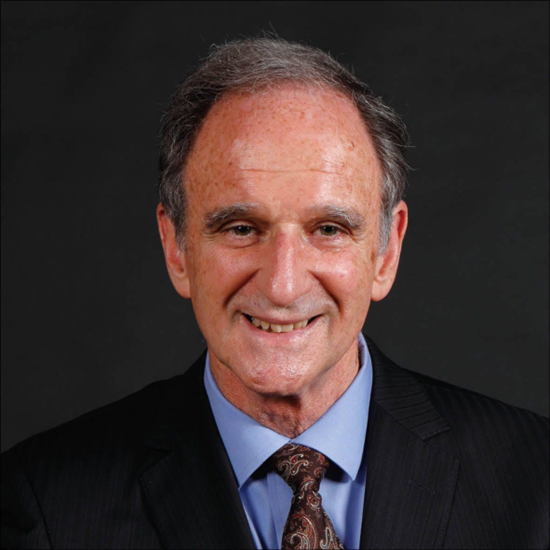
\includegraphics[scale = 0.4]{pictures/Martin_Edward_Hellman.png}
\end{figure}
Martin Edward Hellman\\(sinh 02/10/1945 - 79 tuổi)
\end{column}

\end{columns}
\end{frame}
%%%%%%%%%%%%%%%%%%%%%%%%%%%%%%%%%%%%%%%%%%%%%%%%%%%%%%%

% <!-- Khái niệm -->

% Khái niệm mã hoá khoá công khai

% Mật mã hóa khóa công khai là một dạng mật mã hoá cho phép người sử dụng trao đổi các thông tin mật mà không cần phải trao đổi các khoá chung bí mật trước đó. Điều này được thực hiện bằng cách sử dụng một cặp khóa có quan hệ toán học với nhau là khóa công khai và khoá cá nhân (hay khóa bí mật).

% Mã khoá công khai còn được gọi là mã không đối xứng. Có những thuật toán mật mã khóa bất đối xứng không có tính chất khóa công khai và bí mật như đề cập ở trên mà cả hai khóa (cho mã hóa và giải mã) đều cần phải giữ bí mật.

% Trong mật mã hóa khóa công khai, khóa cá nhân phải được giữ bí mật trong khi khóa công khai được phổ biến công khai. Hai khóa này khác nhau, một dùng để mã hóa và khóa còn lại dùng để giải mã. Điều quan trọng đối với hệ thống là không thể tìm ra khóa bí mật nếu chỉ biết khóa công khai.

% Lưu ý:

% Một hệ mật khóa công khai không bao giờ cung cấp độ mật vô điều kiện - thực tế, đó là hàm cửa sập một chiều (a trapdoor one-way function).

% <!-- -->

% <!-- Mô hình tổng quát -->

% ![alt text](public.png)

% <!-- hệ mật mã khóa công khai bao gồm: bản rõ, bản mã, mã hóa, giải mã, khóa công khai K+ và khóa bí mật K-. hệ mật mã khóa công khai là hệ mật mã bất đối xứng Vì mã hóa và giải mã sử dụng khóa khác nhau -->

% <!-- Giới thiệu về hệ mật mã Rabin -->

%! %%%%%%%%%%%%%%%%%%%%%%%%%%%%%%%%%%%%%%%%%%%%%%%%%%%%%%
%! %%%%%%%%%%%%%%%%%%%%%%%%%%%%%%%%%%%%%%%%%%%%%%%%%%%%%%
%! %%%%%%%%%%%%%%%%%%%%%%%%%%%%%%%%%%%%%%%%%%%%%%%%%%%%%%
%! %%%%%%%%%%%%%%%%%%%%%%%%%%%%%%%%%%%%%%%%%%%%%%%%%%%%%%
%! %%%%%%%%%%%%%%%%%%%%%%%%%%%%%%%%%%%%%%%%%%%%%%%%%%%%%%
\section{Hệ mật mã RSA}
\subsection{xxxxxxxxxxxxxxxxxxxxxx}
\subsubsection{xxxxxxxxxxxxxxxxxxxxxx}
\begin{frame}{xxxxxxxxxxxxxxxxxxxxxx}

\end{frame}
%%%%%%%%%%%%%%%%%%%%%%%%%%%%%%%%%%%%%%%%%%%%%%%%%%%%%%%

%! %%%%%%%%%%%%%%%%%%%%%%%%%%%%%%%%%%%%%%%%%%%%%%%%%%%%%%
%! %%%%%%%%%%%%%%%%%%%%%%%%%%%%%%%%%%%%%%%%%%%%%%%%%%%%%%
%! %%%%%%%%%%%%%%%%%%%%%%%%%%%%%%%%%%%%%%%%%%%%%%%%%%%%%%
%! %%%%%%%%%%%%%%%%%%%%%%%%%%%%%%%%%%%%%%%%%%%%%%%%%%%%%%
%! %%%%%%%%%%%%%%%%%%%%%%%%%%%%%%%%%%%%%%%%%%%%%%%%%%%%%%
\section{Phương pháp lưới và thuật toán LLL giảm lưới}
\subsection{xxxxxxxxxxxxxxxxxxxxxx}
\subsubsection{xxxxxxxxxxxxxxxxxxxxxx}
\begin{frame}{xxxxxxxxxxxxxxxxxxxxxx}

\end{frame}
%%%%%%%%%%%%%%%%%%%%%%%%%%%%%%%%%%%%%%%%%%%%%%%%%%%%%%%
%! %%%%%%%%%%%%%%%%%%%%%%%%%%%%%%%%%%%%%%%%%%%%%%%%%%%%%%
%! %%%%%%%%%%%%%%%%%%%%%%%%%%%%%%%%%%%%%%%%%%%%%%%%%%%%%%
%! %%%%%%%%%%%%%%%%%%%%%%%%%%%%%%%%%%%%%%%%%%%%%%%%%%%%%%
%! %%%%%%%%%%%%%%%%%%%%%%%%%%%%%%%%%%%%%%%%%%%%%%%%%%%%%%
%! %%%%%%%%%%%%%%%%%%%%%%%%%%%%%%%%%%%%%%%%%%%%%%%%%%%%%%
% \section{Tổng kết}
% \subsection{Tổng kết}
% \subsubsection{Tổng kết}
% \begin{frame}{Tổng kết}
% Có cần phần Tổng kết????
% \end{frame}
%%%%%%%%%%%%%%%%%%%%%%%%%%%%%%%%%%%%%%%%%%%%%%%%%%%%%%%

%! %%%%%%%%%%%%%%%%%%%%%%%%%%%%%%%%%%%%%%%%%%%%%%%%%%%%%%
%! %%%%%%%%%%%%%%%%%%%%%%%%%%%%%%%%%%%%%%%%%%%%%%%%%%%%%%
%! %%%%%%%%%%%%%%%%%%%%%%%%%%%%%%%%%%%%%%%%%%%%%%%%%%%%%%
%! %%%%%%%%%%%%%%%%%%%%%%%%%%%%%%%%%%%%%%%%%%%%%%%%%%%%%%
%! %%%%%%%%%%%%%%%%%%%%%%%%%%%%%%%%%%%%%%%%%%%%%%%%%%%%%%
% \section*{}
% \begin{frame}{}
% \centering
% \Huge{Thanks for listening!}
% \end{frame}
%%%%%%%%%%%%%%%%%%%%%%%%%%%%%%%%%%%%%%%%%%%%%%%%%%%%%%%
\end{document}

% \begin{columns}

% \begin{column}{0.4\textwidth}
% \includegraphics[width=\textwidth]{pictures/Giới thiệu về HRM.png}
% \end{column}

% \begin{column}{0.6\textwidth}
% \begin{itemize}
% \item \dots
% \item \dots
% \item \dots
% \end{itemize}
% \end{column}

% \end{columns}